The WR technology \cite{Wlostowski2011} is an international collaborative
project started at CERN in 2009, later joined by other worldwide laboratories and companies. It was born as a replacement technology for CERN's accelerator timing system, but due to its versatility and improved performance compared to other alternatives, together with its open nature, it was quickly adopted by other scientific institutions. In addition to the scientific applications, some private companies such as Seven Solutions or Creotech are interested in extendind WR for industrial solutions. Some examples of that effort are the projects WR-SYNTEF \cite{web:creotech_projects} and IFMIF/EVEDA \cite{web:seven_projects}. 
Furthermore, from its very early stages, WR was launched as an open SW/HW initiative with available online sources at CERN's Open Hardware Repository (OHWR) \cite{ohwr:repo}. This encouraged different companies and research institutions to openly collaborate in its development.

The WR protocol extends PTPv2 with extra messages and has been proposed to be
included in the new PTP release (PTPv3) as High Accuracy (HA) profile
\cite{wr:maciej-ptpv3-standard} . Its main goal is to provide a synchronisation
accuracy better than 1 ns and precision in the scale of ps. The major
improvements introduced by the WR protocol address weak aspects of the PTPv2:
the limitation of the phase difference measurements to one period of the system
clock; and the assumption of symmetry between transmission and reception
paths. It inherently performs self-calibration over optical fibre links and it
is capable of distributing time to a very large number of devices with very
small degradation. Nevertheless, this technology was not designed originally
to address synchronization over long distance links, neither the inclusion of monitoring and dependable mechanisms on the nodes. Although SKA is working on improving both issues, this contribution particularly presents a new platform capable of disseminating the PPS signal incorporating flexibility and dependability features. 

The WR synchronisation mechanisms include the following elements:

\begin{itemize}
	
	\item Frequency synchronisation (syntonization): The recovered clock from the physical layer (L1) of the Open Systems Interconnection model (OSI) is used by 
	the WR logic to syntonize the local oscillator. That means that all the WR network run syntonized with the main clock reference.
	
	\item Phase synchronisation: Thanks to the syntonization, the one-cicle time resolution limitation is resolved via the use of the Dual Mixed Time Difference method (DMTD). A digital implementation of that \cite{Moreira2011} is used to achieve sub-picosecond resolution when measuring phase difference between the local oscillator and the recovered one from the upwards node.
	
	\item Time synchronisation: It is implemented by an enhanced version of the PTPv2 protocol and provides a global notion of time to the entire network. WR 
	also takes into account the asymmetries in the propagation time due to the utilisation of different wavelengths in the same fibre link improving the 
	accuracy of standard PTP protocol. 
\end{itemize}

WR implements mechanisms to ensure deterministic and reliable data transfer between thousand of nodes connected over optical fibre links up to 10 km.
However, it can easily be extended up to 50 km without significant degradation and up to 120 km without the needs of optical amplification. One application of the WR for long links can be found in \cite{Kaur2017}.

\subsection{Network topology} \label{subsec:wr-net}

A typical WR network presents a tree topology and is composed of three different
kind of elements: a Grandmaster (GM), several intermediate devices such as
switches, and end-nodes as shown in the Figure \ref{fig:wr_hierarchy}. The GM
is normally connected to a very stable clock such as an atomic clock or a GPS
receiver \cite{Daniluk2012}. The intermediate levels of the network disseminate
the timing packets to the final nodes, which are composed of other devices such
as WR Switches, WR-ZENs, WR Light Embedded Nodes (WR-LEN) or The Simple PCIe FPGA Mezzannine Card (FMC) carrier (SPEC). These devices have several ports and can behave as PTPv2 Boundary Clocks (BC). Moreover, they are connected using the master-slave scheme: some ports act as slave (upstream) of the to the upper layer while the others are masters (downstreams) and they are in charge of propagating the synchronisation to the next level of the hierarchy. The nodes of the last level of the network are known as slave devices. They recover the clock reference from the link and synchronise their local oscillators in order to provide a time reference for a specific application.

In addition to the conventional tree topology of the timing networks, new
network topologies are currently under-study in WR to add some mechanisms to improve fault
tolerance and security. Examples of this research are
\cite{jlgutierrez-paper-redundancy} and \cite{jlgutierrezhsr} that incorporate Transparent Clocks
(TC) and redundancy protocols to the WR technology such as
High-availability Seamless Redundancy (HSR) to ensure data delivery and reception in critical applications such as
control network, real-time applications or Smart Grids among others.

\begin{figure}[H] \centering 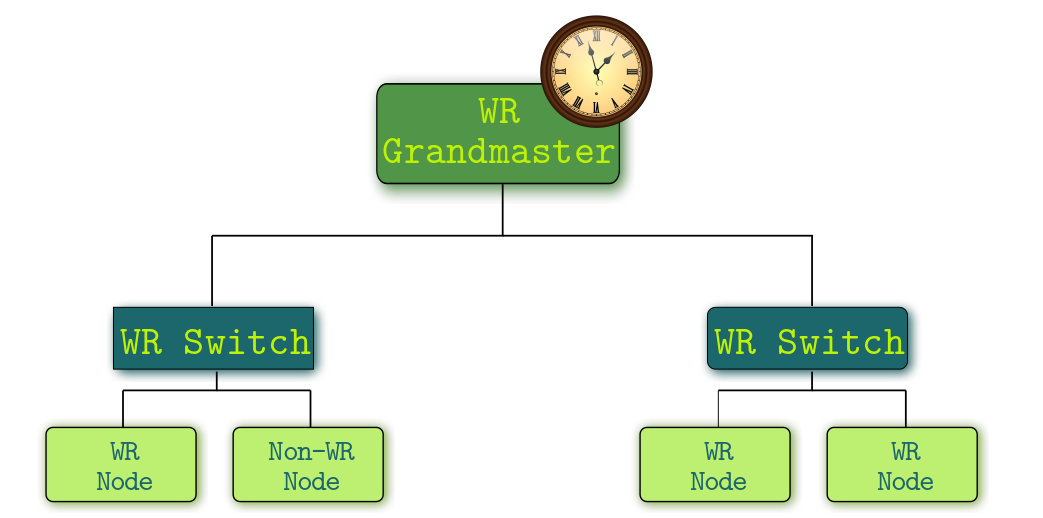
\includegraphics[scale=0.4]{img/wr_hierarchy}
	\caption{The WR network is a tree hierarchy where the root node is the
	GM that is responsible for distributing the reference time signals. The intermediate elements are WRS that acts as Gigabit Ethernet switches and as Boundary Clocks propagating the time signals from the upper layers of the network. Finally, the main purpose of the end-nodes
	is to provide timing to another specific application.}
\label{fig:wr_hierarchy} \end{figure}

\subsection{WR devices survey for the SKA Telescope} \label{subsec:wr-dev}

Regardless of the case of use for the WR technology, it will be needed to select
a suitable set of WR devices. Most applications distinguish between two main roles
according to a typical WR network: devices which act as BC, and those that act as
Ordinary Clocks (OC). Currently, the WRS \cite{ohwr:wrs} is the most convenient
BC among all the WR devices. 

The WRS has a total of 18 Small Form-factor Pluggable (SFP) transceivers, one of which can be configured as slave (upstream) and the rest as masters (downstream). It is also important to remark another I/O ports such as: five coaxial RF connectors and one management Ethernet RJ45 connector. Although there are other WR devices that could act as BC, the WRS is the most appropriate for a network with a high number of nodes, such as is the SKA Telescope, because of its high number of SFP slots.

Nowadays, there  are several WR platforms that can act as OCs. 
For this reason, we have analysed three devices taking into account the specific requirements of the SKA project.

Table \ref{tab:wr_devcomp} contains a comparison between the following three WR
devices: 

\begin{itemize} 
	\item The SPEC \cite{ohwr:spec} is a WR-compliant FMC carrier that supports low pin count (LPC) boards. It includes a Xilinx's Spartan-6 FPGA, a SFP connector and a PCIe interface. It could be used in standalone mode \cite{migueljl-paper-wr-spec}, but due to its limited computational resources, the SPEC is usually used connected to a host PC using the PCIe interface.  No coaxial RF connectors are included in this board, being this fact a major penalty since a FMC board is required to retrieve the PPS signal.
	
	\item The WR Light Embedded Node (LEN) \cite{sevensols:wr_len} is a 	standalone WR node whose main design principles are: an easiness of use and a good timing performance. It was the first WR node	that included the extended version of the WR PTP core (WRPC)architecture, the WR PTP Core Dual Port (WRC2P) \cite{torres2016scalability}. Besides the second WR-compliant Ethernet interface, the WR-LEN includes three coaxial RF
	connectors and a Ethernet RJ45 management port. Its design is quite similar to the SPEC board with some component upgrades, such as the FPGA (Xilinx's Artix-7). This device can act as BC and OC.
	
	\item The WR Zynq Embedded Node (ZEN) \cite{sevensols:wr_zen} is another
	standalone WR node but with many improvements compared to the rest of WR nodes. As in the WR-LEN, the WR implementation corresponds to the WRC2P.  This enables a BC configuration as well as OC, or GM configurations. Design is based on a Xilinx FPGA-SoC (Zynq-7000). It includes a dual ARM core included that enables the utilisation of a Linux-like	OS. The board main I/O connectors are: a FMC high pin count (HPC), two SFPs, five coaxial RF and two Ethernet RJ45. The clocking resources include a low-noise oscillator and a flexible PLL schema.
\end{itemize}

 \begin{threeparttable}\centering \ra{1.1} \begin{tabular}{@{} lccc@{}}%\toprule
	 & \rotatebox[origin=c]{60}{SPEC} & \rotatebox[origin=c]{60}{WR-LEN}  &
	 \rotatebox[origin=c]{60}{WR-ZEN} \\ \midrule \textbf{WR-compliant}\\
	 \tab\small{+BC} & \Circle & \CIRCLE & \CIRCLE \\ \tab\small{+OC} &
	 \CIRCLE & \CIRCLE & \CIRCLE \\ \tab\small{+GM} & \LEFTcircle &
	 \LEFTcircle & \CIRCLE \\ \tab\small{+Standalone} & \LEFTcircle &
	 \CIRCLE & \CIRCLE \\
		
		\textbf{RF interfacing}\\ \tab\small{+PPS output} & \LEFTcircle
		& \CIRCLE & \CIRCLE \\ \tab\small{+RF I/O} & \Circle & \CIRCLE &
		\CIRCLE \\ \tab\small{+GM input} & \LEFTcircle & \LEFTcircle &
		\CIRCLE \\
		
		\textbf{Dev. support}\\ \tab\small{+Monitoring support} &
		\LEFTcircle & \LEFTcircle & \CIRCLE  \\ \tab\small{+Linux OS} &
		\Circle & \Circle & \CIRCLE \\ \tab\small{+Available resources}
		& \LEFTcircle & \Circle & \CIRCLE \\
		
		\textbf{Extensions}\\ \tab\small{+FMC connector} & \LEFTcircle &
 \Circle & \CIRCLE \\ \tab\small{+Redundancy} & \Circle & \LEFTcircle &
 \LEFTcircle \\ \bottomrule \end{tabular} \begin{tablenotes} \item \hfill
		 \small{\CIRCLE Fully supported; \LEFTcircle Partially
 supported; \Circle Not supported} \end{tablenotes} \caption{Comparison between
 three WR nodes.} \label{tab:wr_devcomp} \end{threeparttable}

Among other WR nodes, the WR-ZEN has been the chosen development platform for the
SKA Telescope PPS system due to its flexibility and main features. The possibility of being used as a standalone node
with Linux support, the inclusion of enough I/O ports (RF, FMC, etc.), together with an improved clocking resources
looks to fulfil the timing requirements of the project.

Next section describes the proposed PPS distribution system for SKA Telescope.